%  5 关系展示 本节主要讲relation的表现方式。
\section{Relationship Display} 
%为了选择效果好的可视化元素来展示实体间关系,我们在一定的限制框架下进行了头脑风暴。经过讨论产生了几种设计案例。根据这几种案例,我们提出了一种设计空间。最后进行了用户调研对它们进行评价。
\noindent In order to select effective visualization elements to show the relationships between entities, we brainstormed within a certain restrictive framework. Several design cases were generated after discussion. Based on these cases, we suggested a design space. Finally a user research was conducted to evaluate them. 
\subsection{Design Cases} %设计案例
% 我们邀请了可视化领域的3位硕士研究生和1位博士生进行了关系展示的头脑风暴。经过独立的分析,我们收集到数份设计图。对它们提炼后,得到了如下几种图例。箭头:;基础图形:;渐变:。
\noindent We invited three master students and one PhD student in the field of visualization to brainstorm relationship presentations. Several design drawings were collected after independent analysis. Distilling them, the following figure legends were obtained.
\ding{172} Arrows: " \raisebox{-0.75mm}{
\includegraphics[scale=0.15]{Fig/arrow.png}} "; 
\ding{173} Basic shape: " \raisebox{-0.75mm}{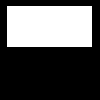
\includegraphics[scale=0.15]{Fig/bg1.png}} ", " \raisebox{-0.75mm}{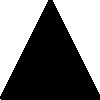
\includegraphics[scale=0.15]{Fig/bg2.png}} ", " \raisebox{-0.75mm}{
\includegraphics[scale=0.15]{Fig/bg3.png}} "; 
\ding{174} Color gradient: "\raisebox{-0.75mm}{
\includegraphics[scale=0.15]{Fig/jianbian.png}}".

%在这些图例中,都存在指向性,即关系中的"施者->受者"。在箭头图例中,方向由箭头隐喻;在基础图形中,由矩形中的颜色(有颜色到无颜色),三角形的顶点方向,半圆的朝向隐喻;在颜色渐变中,由颜色从深到浅隐喻。
In all these figure legends, there is directionality, i.e., "\textit{giver} $\rightarrow$ \textit{receiver}" in the SPO triple. In \ding{172}, the direction is metaphorically represented by the arrow; in \ding{173}, by the color in the rectangle (colored to uncolored), the direction of the vertices of the triangle, and the orientation of the semicircle; in \ding{174}, by the color from dark to light.

%经过参与者的讨论,我们发现,上述图例之间的组合形成的效果也很好。例如将箭头与基础图形结合可以得到:···;同理,将基础图形与颜色渐变结合可以得到:···。我们使用上述图例制作了一些设计案例:
Through the discussion of the participants, we found that the combination between the above figure legends formed a good effect as well. \ding{175} hybridizing the arrows with the base shapes yields: " \raisebox{-1mm}{
\includegraphics[scale=0.15]{Fig/mixabg1.png}} ", " \raisebox{-1mm}{
\includegraphics[scale=0.15]{Fig/mixabg3.png}} ". Similarly, \ding{176} hybridizing the base shapes with the color gradient yields: " \raisebox{-1mm}{
\includegraphics[scale=0.15]{Fig/mixcbg1.png}} ", " \raisebox{-1mm}{
\includegraphics[scale=0.15]{Fig/mixcbg2.png}} ", " \raisebox{-1mm}{
\includegraphics[scale=0.15]{Fig/mixcbg3.png}} ".
We have produced some design cases using the above figure legend.

%案例
\begin{figure}[h]
	\begin{minipage}{0.24\linewidth}
		\centerline{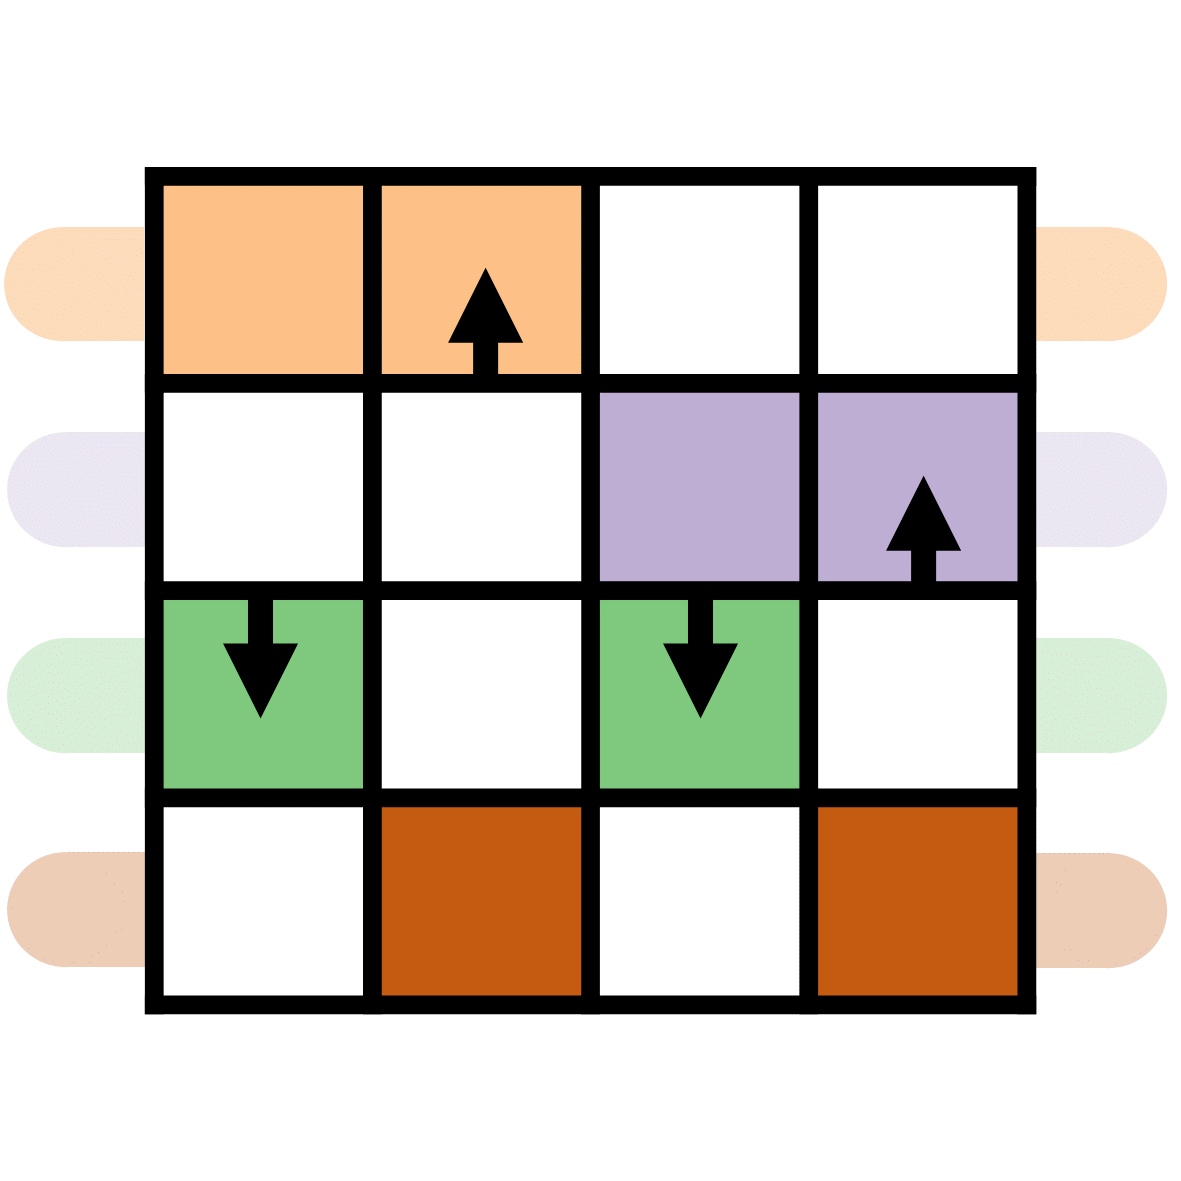
\includegraphics[width=\textwidth]{Fig/11.png}}
		\vspace{-1pt}
		\centerline{(a).1}
		\centerline{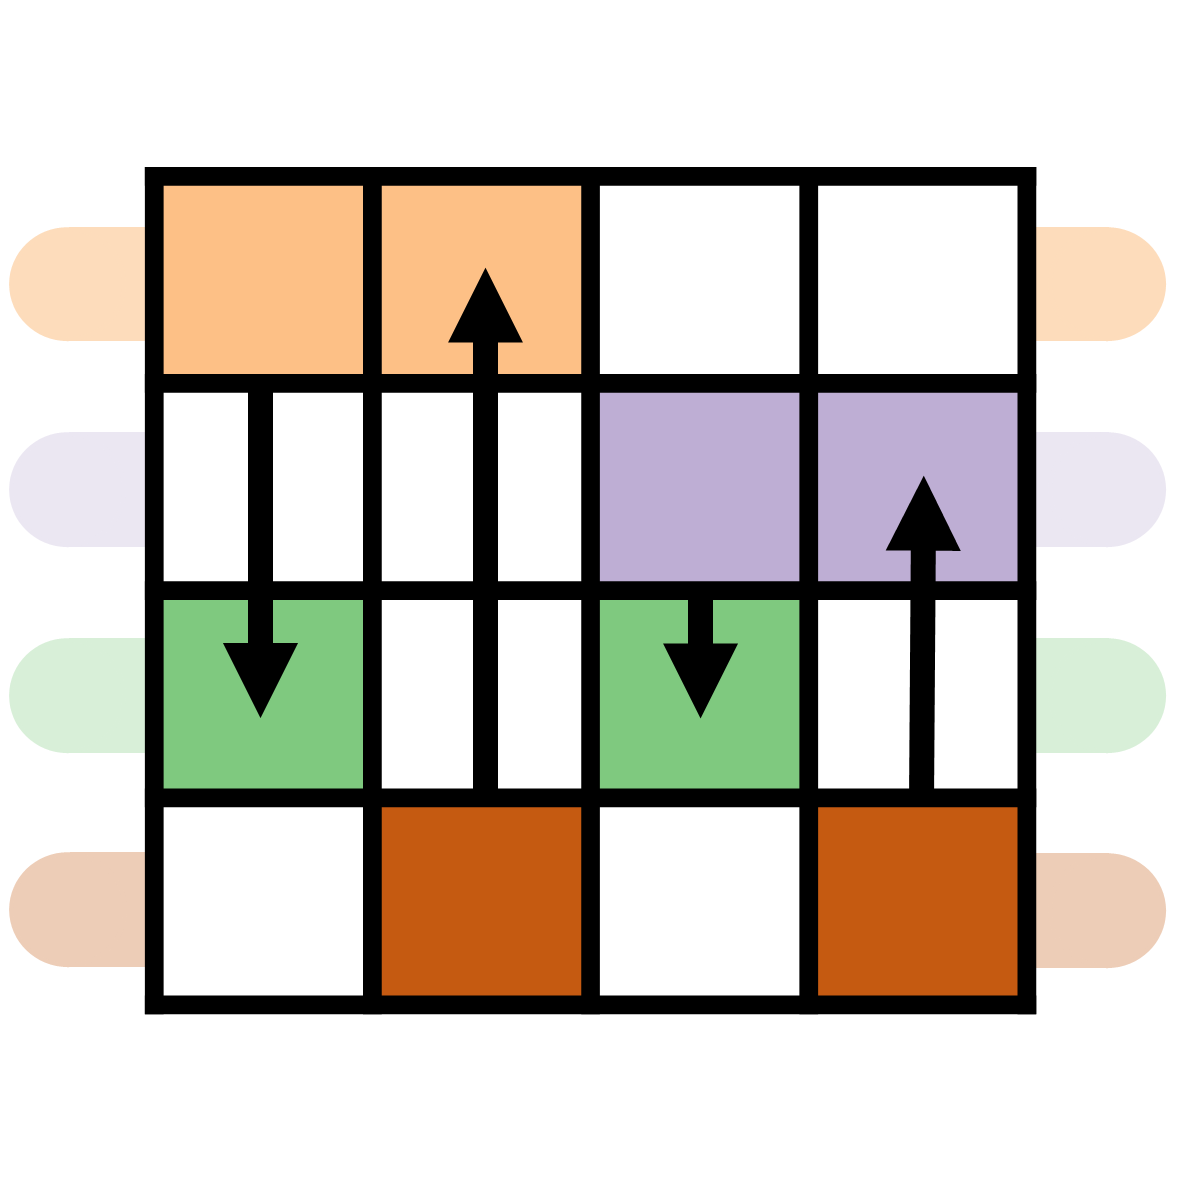
\includegraphics[width=\textwidth]{Fig/12.png}}
		\vspace{-1pt}
		\centerline{(a).2}	
		\centerline{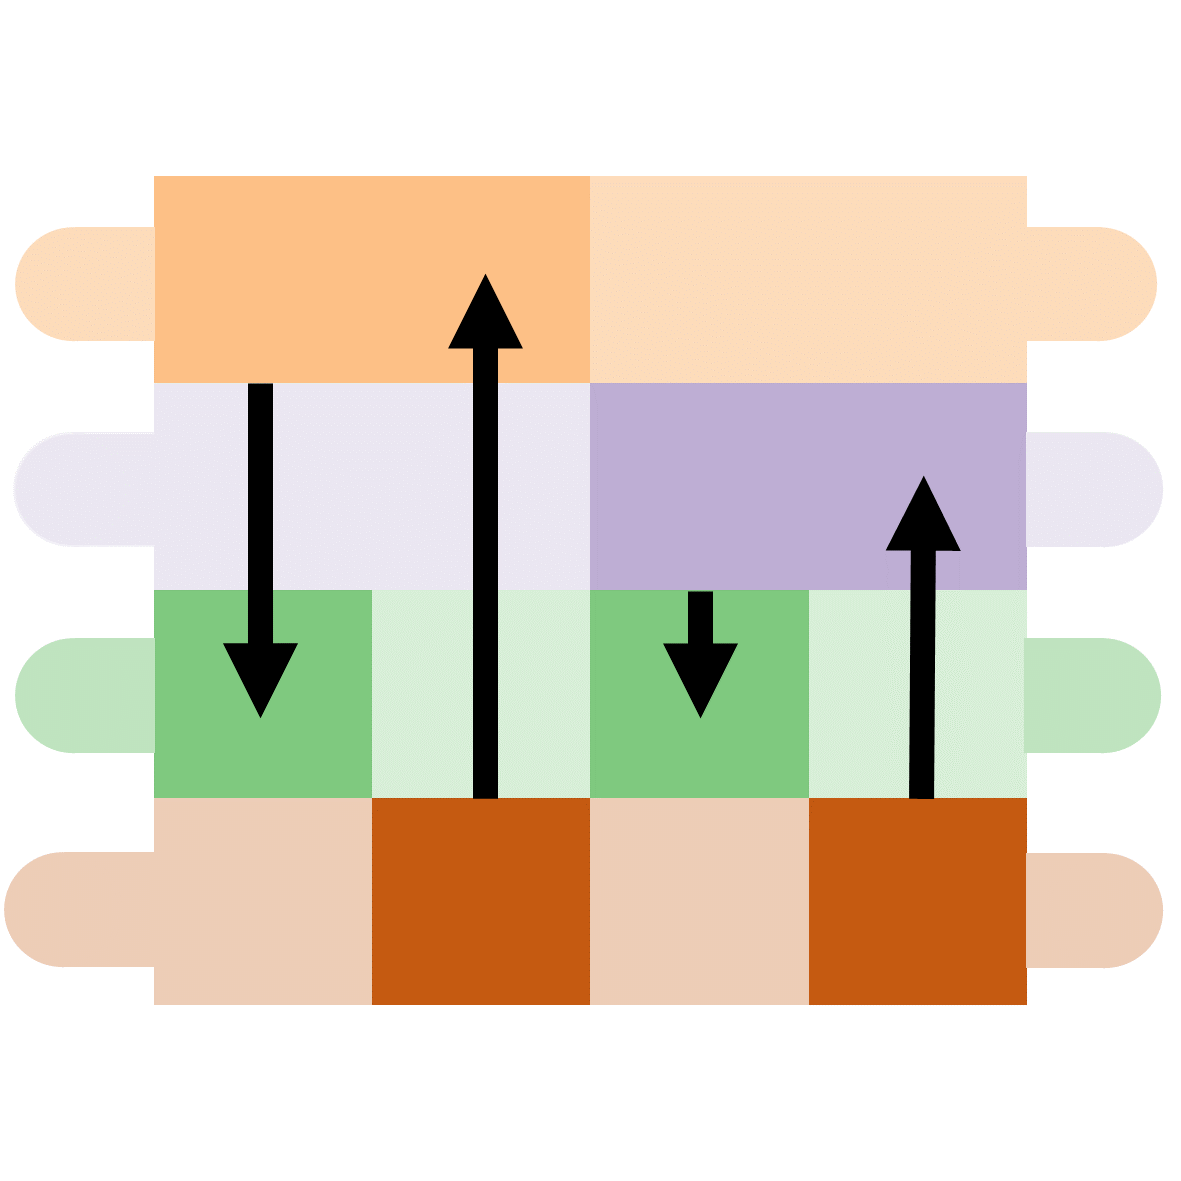
\includegraphics[width=\textwidth]{Fig/13.png}}
		\vspace{-1pt}
		\centerline{(a).3}
	\end{minipage}
	\begin{minipage}{0.24\linewidth}
		\centerline{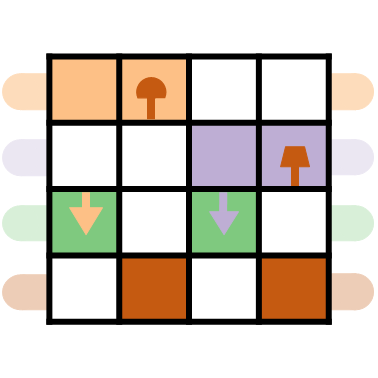
\includegraphics[width=\textwidth]{Fig/21.png}}
		\vspace{-1pt}
		\centerline{(b).1}
		\centerline{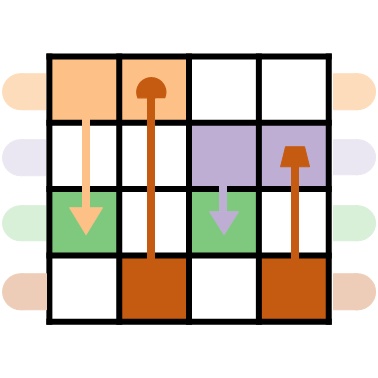
\includegraphics[width=\textwidth]{Fig/22.png}}
		\vspace{-1pt}
		\centerline{(b).2}
		\centerline{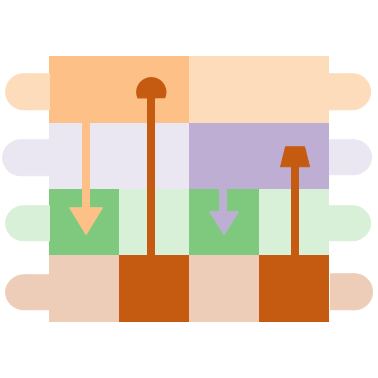
\includegraphics[width=\textwidth]{Fig/23.png}}
		\vspace{-1pt}
		\centerline{(b).3}
	\end{minipage}
	\begin{minipage}{0.24\linewidth}
		\centerline{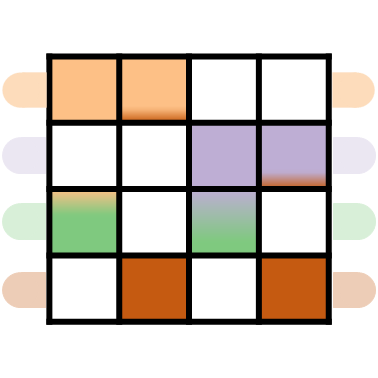
\includegraphics[width=\textwidth]{Fig/31.png}}
		\vspace{-1pt}
		\centerline{(c).1}
		\centerline{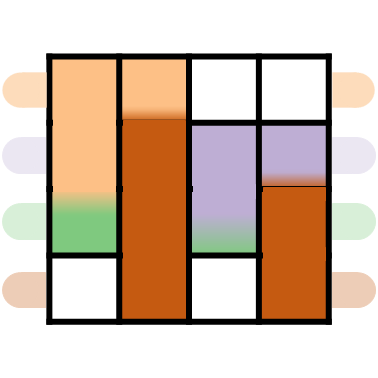
\includegraphics[width=\textwidth]{Fig/32.png}}
		\vspace{-1 pt}
		\centerline{(c).2}
		\centerline{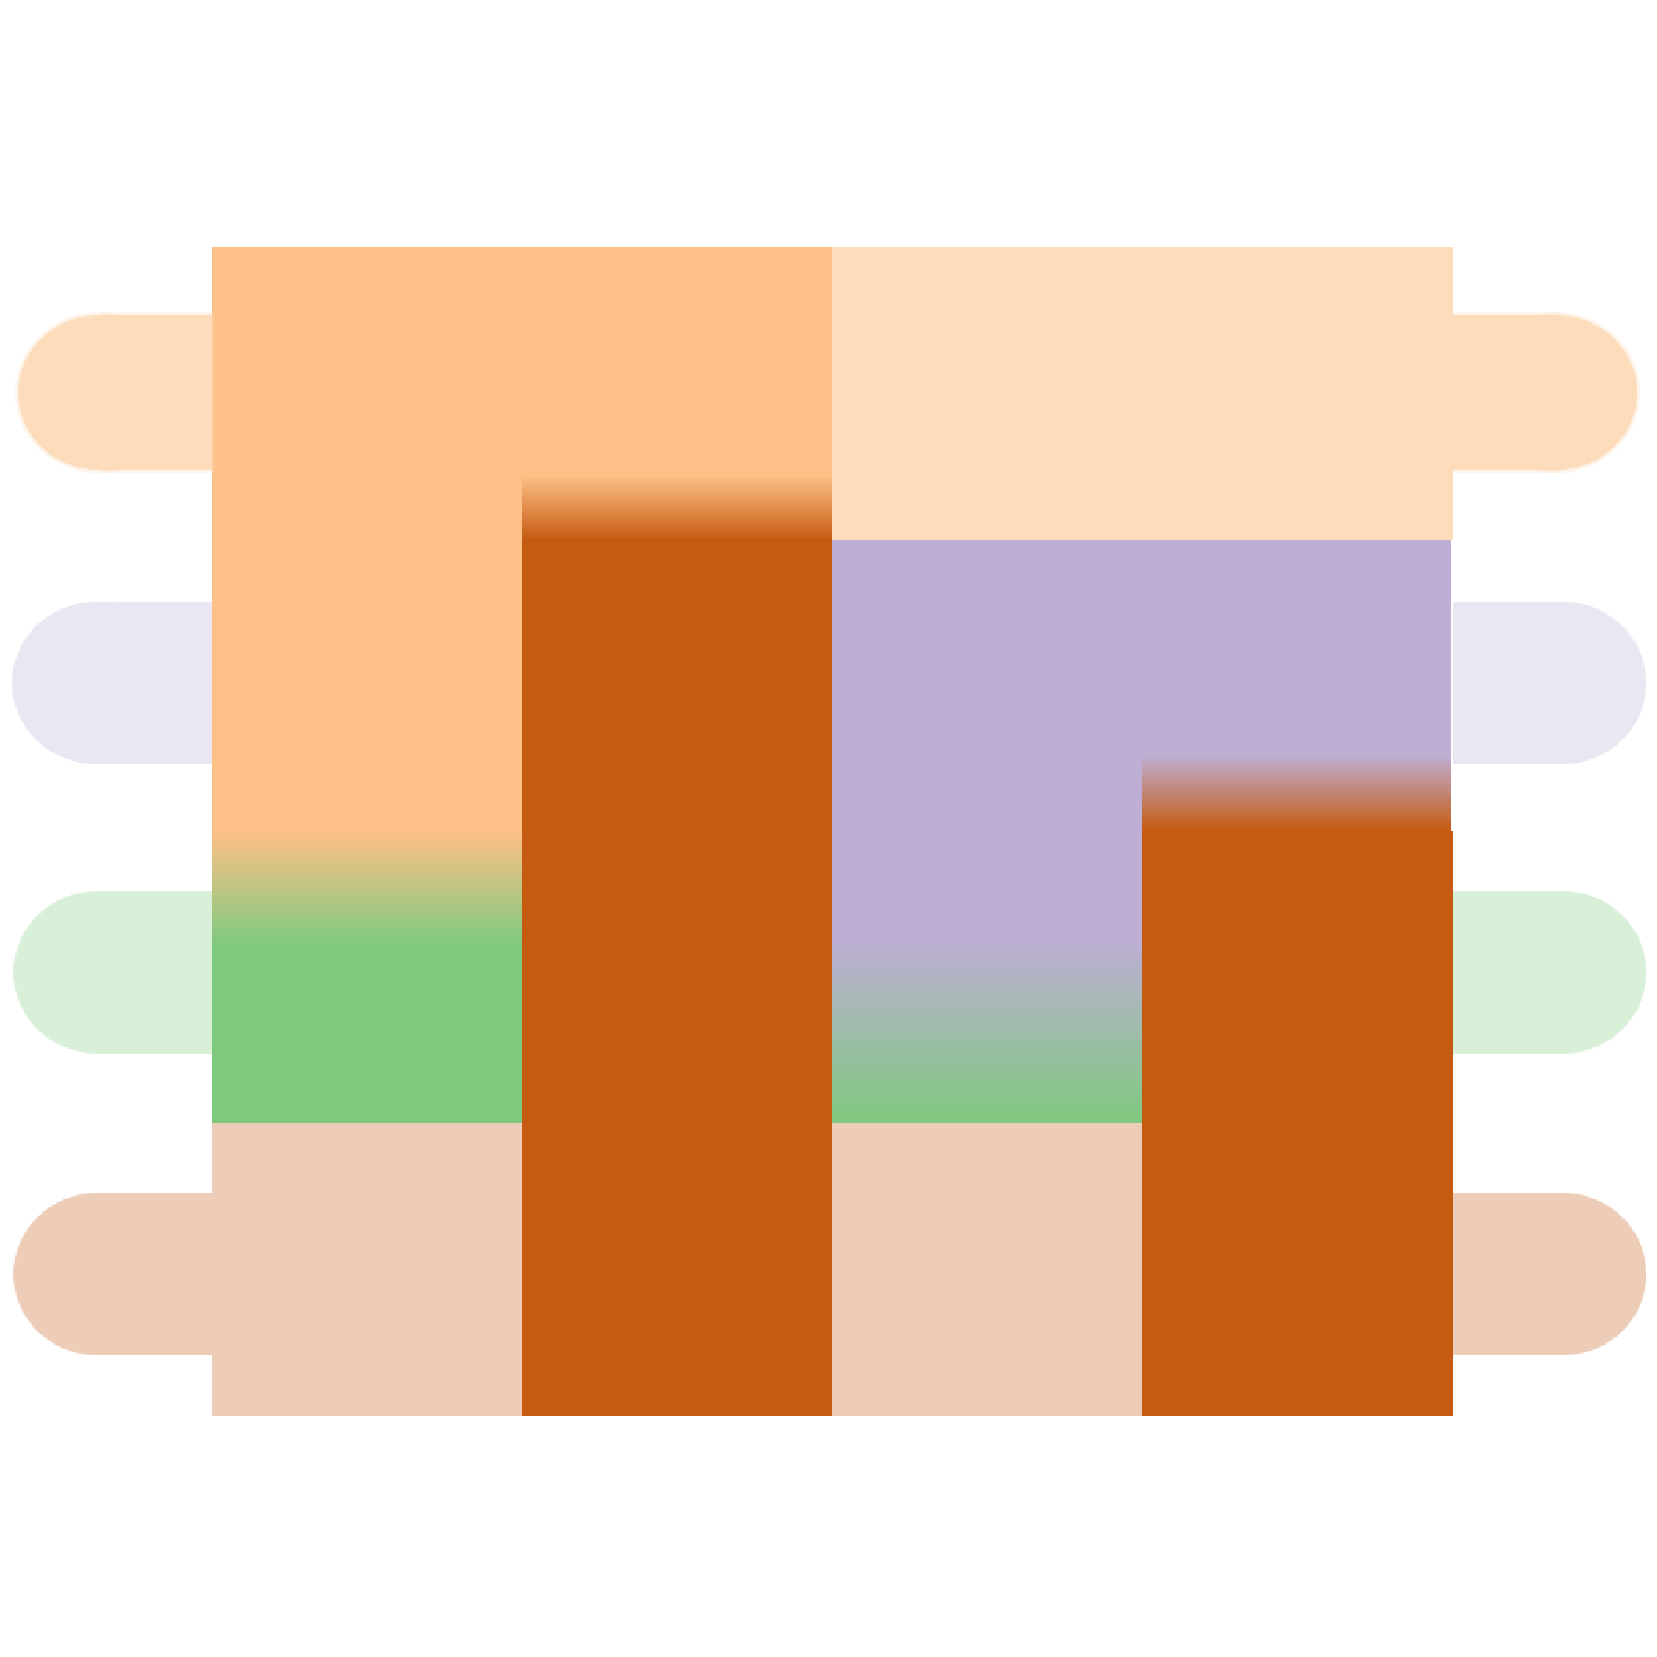
\includegraphics[width=\textwidth]{Fig/33.png}}
		\vspace{-1pt}
		\centerline{(c).3}
	\end{minipage}
	\begin{minipage}{0.24\linewidth}
		\centerline{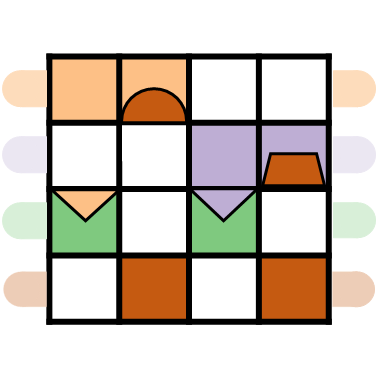
\includegraphics[width=\textwidth]{Fig/41.png}}
		\vspace{-1pt}
		\centerline{(d).1}
		\centerline{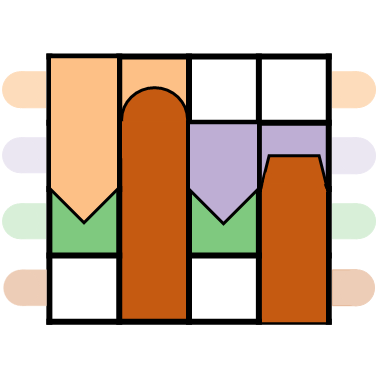
\includegraphics[width=\textwidth]{Fig/42.png}}
		\vspace{-1pt}
		\centerline{(d).2}
		\centerline{
\includegraphics[width=\textwidth]{Fig/43.png}}
		\vspace{-1pt}
		\centerline{(d).3}
	\end{minipage}
	\caption{Design cases. (a)arrows; (b)arrows + base shapes; (c)color gradient; (d)color gradient + base shapes.}
	\label{fig:DC}
\end{figure}

%图6为设计案例的示意图。图6.a中的图例为箭头,图6.b中的图例为箭头+基础形状,图6.c中的图例为颜色渐变,图6.d中的图例为基础形状+颜色渐变。我们提出了一个设计空间,用来评判设计案例的功能。设计空间中的评价指标有:\ding{183}是否能展示实体间具有关系,\ding{184}是否能区分关系的施者与受者,\ding{185}是否能展示关系属性。
Fig~\ref{fig:DC} shows design case schematics, where the legends used are arrow, arrow + base shape, color gradient, and base shape + color gradient. We propose a design space for judging the functionality of each design case. The evaluation metrics in the design space are: \ding{183} whether the entity relationship can be demonstrated, \ding{184} whether the giver and the receiver of the relationship can be distinguished, and \ding{185} whether the relationship properties can be demonstrated.

%表格绘制
\renewcommand{\arraystretch}{2}
\newcolumntype{Y}{>{\centering\arraybackslash}X}
\begin{table}[h]
	\label{key}
	\centering
	\begin{tabularx}{0.5\textwidth}{| c | Y | Y | Y | Y |}
		\hline
		\multicolumn{2}{|c|}{\multirow{2}{*}{Design Cases}} & \multicolumn{3}{c|}{Evaluation Metrics}  \\ 
		\cline{3-5}
		\multicolumn{2}{|p{3cm}|}{\centering}                              
		& whether the entity relationship can be demonstrated & whether the giver and the receiver of the relationship can be distinguished & whether the relationship properties can be demonstrated                       \\ 
		\hline
		\multirow{3}{*}{a} {\centering}
		& 1    & \checkmark &   &                          \\ 
		\cline{2-5}
		& 2    & \checkmark &   &                          \\ 
		\cline{2-5}
		& 3    & \checkmark &   &                          \\ 
		\hline
		\multirow{3}{*}{b} 
		& 1    & \checkmark & \checkmark & \checkmark                        \\ 
		\cline{2-5}
		& 2    & \checkmark & \checkmark & \checkmark                        \\ 
		\cline{2-5}
		& 3    & \checkmark & \checkmark & \checkmark                        \\ 
		\hline
		\multirow{3}{*}{c} 
		& 1    & \checkmark & \checkmark &                          \\ 
		\cline{2-5}
		& 2    & \checkmark & \checkmark &                          \\ 
		\cline{2-5}
		& 3    & \checkmark & \checkmark &                          \\ 
		\hline
		\multirow{3}{*}{d} 
		& 1    & \checkmark & \checkmark & \checkmark                        \\ 
		\cline{2-5}
		& 2    & \checkmark & \checkmark & \checkmark                        \\ 
		\cline{2-5}
		& 3    & \checkmark & \checkmark & \checkmark                        \\
		\hline
	\end{tabularx}
\end{table}

%用户调研
\subsection{User Studis}
%
\noindent